\documentclass[newfonts=false,format=sigconf,10pt,letterpaper]{acmart}
\usepackage{times}
\usepackage{geometry}
% for document class article
\usepackage{epsfig}
\usepackage{amssymb}
\usepackage{amsmath}
\usepackage{amsfonts}

\usepackage{graphicx}
\usepackage{stackengine}
\usepackage{subfigure}
\usepackage{algorithmic,comment}
\usepackage[ruled,vlined,commentsnumbered,titlenotnumbered]{algorithm2e}
\usepackage{float}
\usepackage{pbox}

% from online
\usepackage{xcolor}
\newcommand\mycommfont[1]{\footnotesize\ttfamily\textcolor{blue}{#1}}
\SetCommentSty{mycommfont}

\usepackage{colortbl}
\usepackage{xcolor}
\definecolor{LightCyan}{rgb}{0.88,1,1}


%% Color text for in situ comments:
\usepackage{color}
\newcommand{\SC}[1]{{\color{blue}#1}}
\newcommand{\tu}[1]{{\underline{\textit{#1}}}}

% Changes to algorithm formatting
\renewcommand{\algorithmiccomment}[1]{ //#1}
\newcommand{\norm}[1]{\left\lVert#1\right\rVert}

\newtheorem{definition}{Definition}
\newtheorem{remark}{Remark}

 
\usepackage{hyperref}
\usepackage{balance}

\hypersetup{pdfstartview=FitH,pdfpagelayout=SinglePage}

\setlength\paperheight {11in}
\setlength\paperwidth {8.5in}
\setlength{\textwidth}{7in}
\setlength{\textheight}{9.25in}
\setlength{\oddsidemargin}{-.25in}
\setlength{\evensidemargin}{-.25in}

\topmargin -0.5in
\headheight 0pt
\textheight 9.25in
\settopmatter{printacmref=false}
\fancyhead{}

\begin{document}

%%%%%%%%%%%%%  ABSTRACT GOES HERE %%%%%%%%%%%%%%
%\begin{abstract}
%	\label{sec:abstract}
%	%\input{sections/abstract.tex}
%\end{abstract}

%%%%%%%%%%%% THIS IS WHERE WE PUT IN THE TITLE AND AUTHORS %%%%%%%%%%%%
\title{Graph Analysis of Major League Soccer Networks: CS224W Final Project}

\author{Evan Huang}
\affiliation{%
	\institution{Stanford University}
}
\email{ehuang@stanford.edu}

\author{Sandeep P. Chinchali}
\affiliation{%
	\institution{Stanford University}
}
\email{csandeep@stanford.edu}

\maketitle

%%%%%%%%%%%%%  INTRO %%%%%%%%%%%%%%
\section{Introduction}
%%%%%%%%%%%%%%%%%%%%%%%%%%
\label{sec:introduction}
Given the natural existence of networks in team-based sports, we hope to use network analysis and predictive modeling to better analyze soccer. Currently, research in soccer analytics has focused on individual player statistics, and predictive modeling has been limited to simple logistic regression, decision trees, and LSTMs [3]. We believe that leveraging network structure will create better results given the importance of teamwork within the sport. In particular, a better predictive model can benefit both the sports betting industry (last year, the total betting on sport was \$4.9 billion in Nevada alone [1]) and the soccer team's management.  




\section{Related Work}
%%%%%%%%%%%%%%%%%%%%%%%%%%
\label{sec:related_work}
One of our main novel contributions in this project would be assessing whether graph-based learning algorithms like Graph Convolutional Networks (GCNs) [2] perform better than other traditional learning algorithms in the context of prediction and analysis of sports games. 

There has been some related work in sports analytics conferences like the MIT Sloan Sports Analytics conference; for example, one paper [3] describes data-driven ghosting in soccer games which enables coaches and managers to “scalably quantify, analyze and compare fine grained defensive behavior”. Their learning task was different than our proposed one here because they were more interested in analyzing and modeling player movements and defense styles, not predicting game statistics. Other related work includes an MIT Master's Thesis [4]  and a journal paper [5] which also use similar data from soccer games to infer passing patterns and styles [4], assess players’ passing effectiveness, and predict shots [5]. However, to the best of our knowledge, none of these papers represent the data as a network graph and utilize the graph structure in their inferences, which is where our current work is situated. 



\section{Dataset and Graph Structure}
%%%%%%%%%%%%%%%%%%%%%%%%%%
\label{sec:dataset}
Our dataset consists of 6 seasons of ``play-by-play'' soccer games from major professional leagues such as Li Liga (Spain), English Premier League (EPL), and Major League Soccer (MLS). For a given game between two teams, ``play-by-play'' data identifies each player, their x and y coordinates in the field, a timestamp of hour, minute, and second, and the major action taken by that player, such as a pass, interception, aerial shot, goal etc. in a standardized vocabulary. 

We collected the annotated data from OPTA, a sports analytics company, which ensured data fidelity and annotated player actions (passing, aerial shots) using uniform video annotation techniques. Overall, the dataset consists of 2,280 games from  players across 60 diverse teams, leading to  3,893,304 player actions (rows). Since only one player is considered in each timestep, we can identify player A passed to player B by considering the action and players in successive timestamps.  

\subsection{EPL Dataset}
To prototype our methods, we have only tested our analysis on the EPL dataset.
For the final project, we will repeat the analysis for all leagues, cluster playing styles across leagues, and compare node feature vectors between leagues.

The EPL dataset consists of a single season in 2012, consisting of 380 matches between 20 teams, such as Liverpool, Manchester United, Southampton, etc. The dataset consists of 648,883 unique plays made by 524 unique players, who are annotated to have 5 positions of Strikers, Defenders, Midfielders, Goalkeepers, and Substitutes. Each play is annotated using a standardized vocabulary of 46 actions, including `Goals' and `Interceptions'.


\subsection{Graph Structure}
The team structure within a given match is represented as a weighted, directed graph, where nodes are players and edges are actions (pass, kick, etc.). Our initial networks also include additional event nodes to represent non-player states such as the gaining of the ball, the loss of a possession, and a shot taken. Respectively these are named ``Gain'', ``Loss'', ``Shot'', and ``Goal''. 

\tu{Nodes:}  14 to 17 nodes consist of 11 players from each team plus events and substitute players. As of now we encode no additional information on the nodes except for ID, but will eventually add in position, location, and time played. 

\tu{Edges:} Actions between states where the ball is located. If player (node) A passed to player (node B) some amount of times within a game, a passing edge is created. Concurrently, shot, gain, and loss rates are also used to connect player nodes to event nodes. The weights on the edges can be formulated as follows: 

\begin{enumerate}

    \item Passes (A, B) = (num. successful passes between A and B) / (time shared between A and B)

    \item Shots(A) = (num. saved attempts, post hits, misses, or goals) / (time A on field) 

    \item Gain(A) = (num. of ball recoveries, corners awarded, out of bounds rewarded) / (time A on field) 

    \item Loss(A) = (num. unsuccessful passes, out of bounds, dispossessions) / (time A on field) 

\end{enumerate}


\begin{figure}[h]
  \centering
  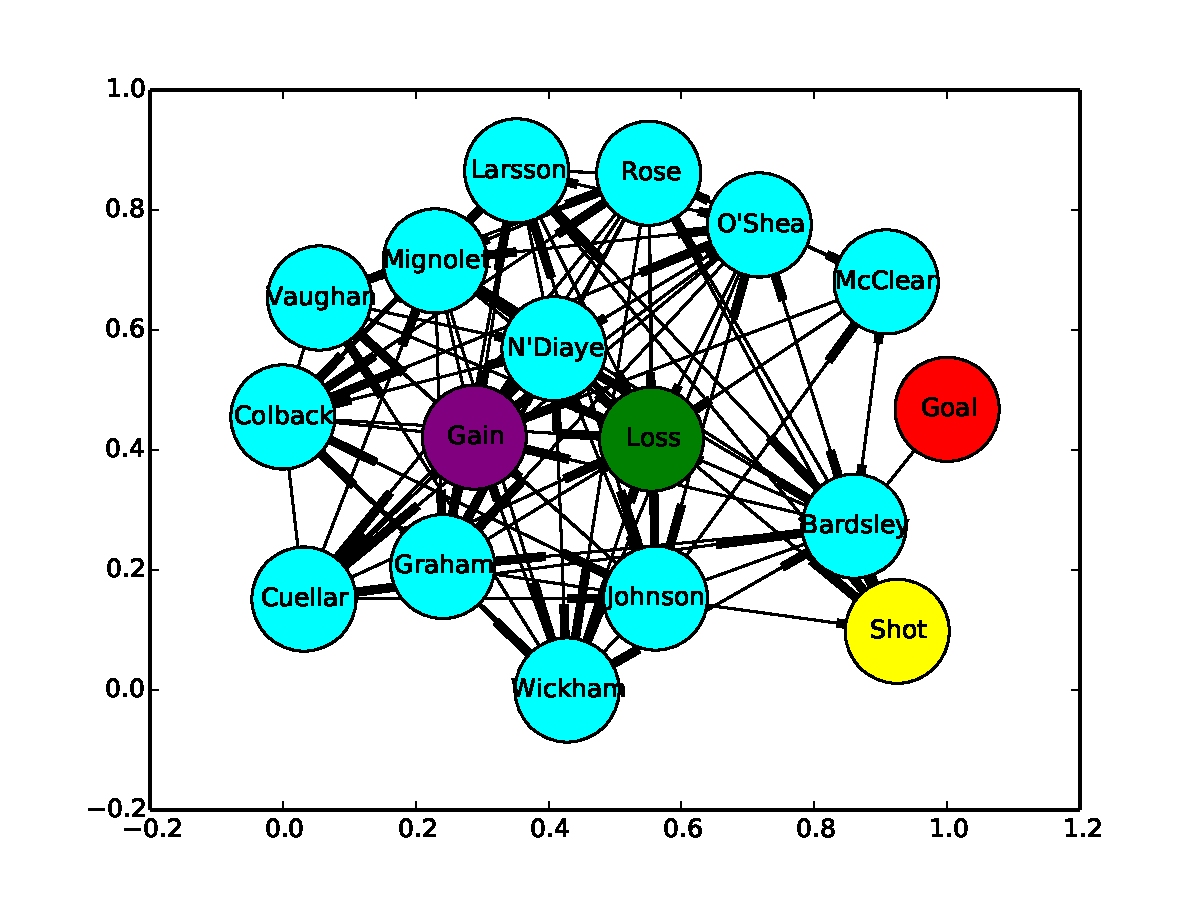
\includegraphics[width=0.45\textwidth]{plots/soccer_networkx.pdf}
  \caption{Example Graph Structure for a Single Team in a Single Game. Player nodes are colored in cyan and edge weights (passing rates) are omitted for visual clarity.}
\end{figure}


\begin{figure}[h]
  \centering
  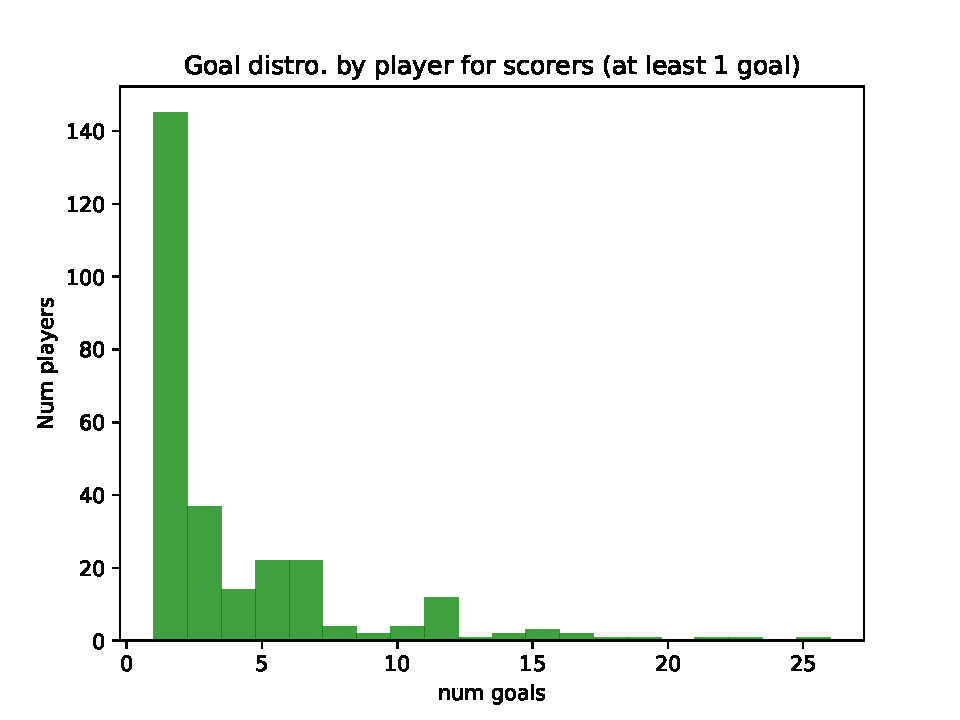
\includegraphics[width=0.45\textwidth]{plots/eplper_player_goal_hist.pdf}
  \caption{Per-player goal distribution across a season.}
\end{figure}



Networks currently in production represent a single team in a single game, such as:

\begin{enumerate}
    \item Single game networks with 2 teams. Each team is connected through respective losses and gains of possessions, transforming original ``Gain'' and ``Loss'' nodes into ``Switch'' nodes.

    \item Aggregated team network consisting of data within a whole season. Each team's individual networks is aggregated across all games, giving one unique network per team. Rates are now based on total time rather time in a game. 
\end{enumerate}

\subsection{Data Processing}

Our initial code processes the play-by-play using 2 pointers that track players making actions, and players receiving actions. Time on field is measured through substitution events, where in the event a substitution doesn’t occur, the player is assumed to have played the whole game. These counts of actions are stored in a dictionary representing an edge list where keys are tuples of player IDs. The time metrics are then used to transform these dictionary components into rates. Additional information tracked include team, home vs away status, goals, winning team, and match id. 

As a sanity check, we plotted the distribution of goals across a season for EPL players that scored at least once. Figure 2 shows a reasonable distribution between 1 goal (the mode) and a maximum of 26 per-player season goals. The edge list dictionary is used to create a passing-rate weighted TNEANet graph in snap. 






\section{Graph Analysis}
%%%%%%%%%%%%%%%%%%%%%%%%%%
\label{sec:graph_analysis}
\begin{figure*}[h]
  \centering
  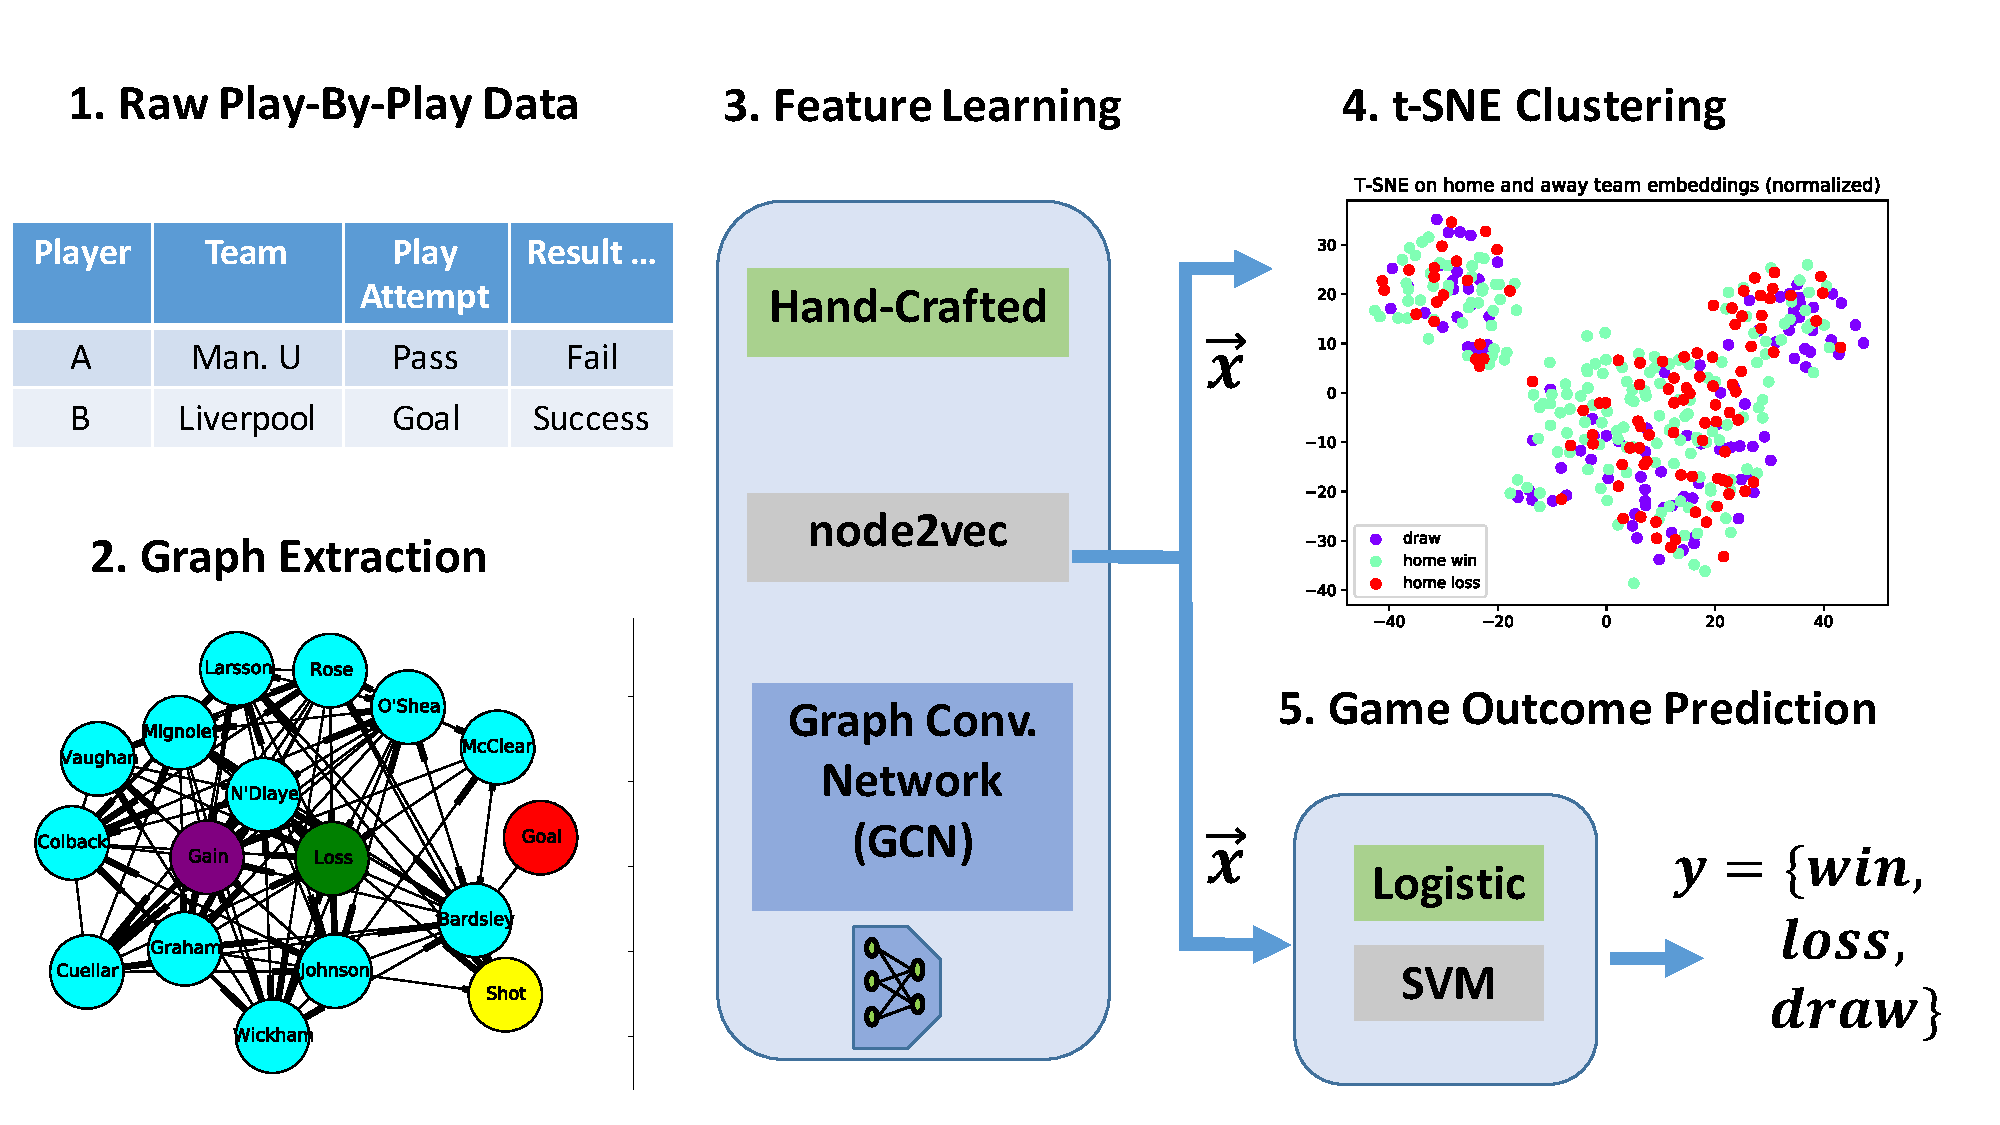
\includegraphics[width=0.95\textwidth]{plots/soccer_block_diagram.pdf}
  \caption{Soccer network analysis pipeline starting from (1) play-by-play data, (2) passing rate graph extraction, (3) feature embedding, (4) clustering, and finally (5) game result prediction. We compared the predictive utility of simple, domain-specific features with complex ones learned by Graph Convolutional Networks (GCNs).}
  \label{fig:block_diagram}
\end{figure*}

\subsection{Feature Learning: Node Embeddings}
Given our goal to predict game results and/or analyze teams effectively, we want to learn node embeddings from our graphs that maximimize predictive and discriminative power.

Our first embedding, which we call simple or hand-crafted features, sets the average pass rate, max pass rate, min pass rate (nonzero), shot rate, gain rate, and loss rate in a vector for each node. We then can assemble a feature vector for a specific graph by averaging the features of the node within the graph. 

Our second embedding uses node2vec [7] with default parameters (128 dimensions, 80 length walk, 10 walks per source, weighted directed graph) to retrieve a feature vector per node. The feature vectors are then averaged to obtain a feature vector for a graph. 

Our current node aggregation technique is simple, but may lose a lot of information. 
Therefore, we hope to learn more rich, higher-order interactions between players, using a more complex model such as a  GCN [2,6].

\subsection{Graph Clustering Based on Feature Vectors}
Given both simple hand-crafted features and those from node2vec per team, we wish to cluster them to discover latent relationships or whether they aggregate based on outcome (`win', `loss', `draw') or team identity. Since each team plays 20 games, we have several realizations of a team's playing style.

We used the standard t-SNE method [9] for clustering since it can be projected to two dimensions for easy visualization. Further, its probabilistic assignment of cluster membership is attractive in the soccer context since teams likely have dynamic playing styles based on their opponent, current substitutions, and even whether they are the home team.

We implemented t-SNE using python's  sklearn package and visualized the embeddings in two dimensions for both simple and node2vec features. Per feature set, we ran t-SNE twice, once on a matrix where rows were matches and columns where a single team's features, and again where rows were matches and columns concatenated both the home and away team's vectors. The latter is more useful to predict outcome since it contrasts the playing style of both teams.

We rigorously applied t-SNE using best practices such as sample normalization to account for the different scales of input variables. Initially, we found a few clusters, though they did not separate based on our desired goal of predicting game outcome.


Upon further analysis of nodes in each cluster, we realized that the clusters corresponded to cases where teams had 14,15,16, or 17 players overall due to substitutions. Also, we sometimes saw two clusters, which were later learned to be for `home' and `away' games but were still not predictive of game result. Examples of such uninformative clusters are provided below. 

\begin{figure}[h]
  \centering
  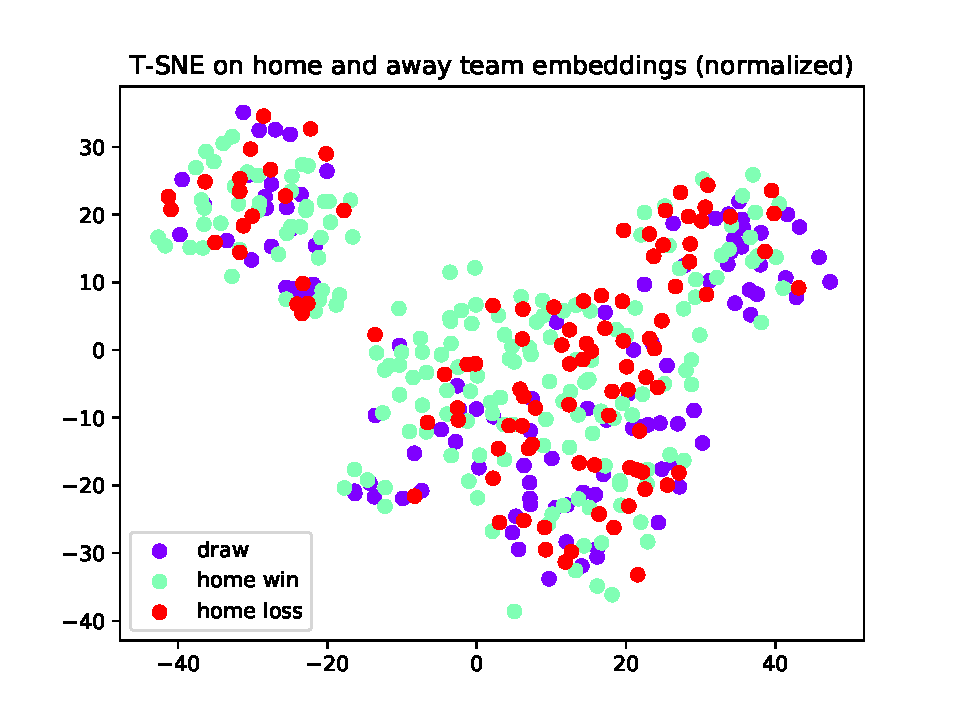
\includegraphics[width=0.45\textwidth]{plots/game_NORM_tsne.pdf}
  \caption{T-SNE shows uninformative clusters based on number of players and home/away status.}
    \label{fig:tsne_game}
\end{figure}


However, when omitting number of players or home/away team status, we realized t-SNE did not help in clustering the data, as shown below. 
Crucially, rather than simply averaging individual player feature vectors, we 
will subsequently learn more predictive features from them using GCNs.


\begin{figure}[h]
  \label{fig:tsne}
  \centering
  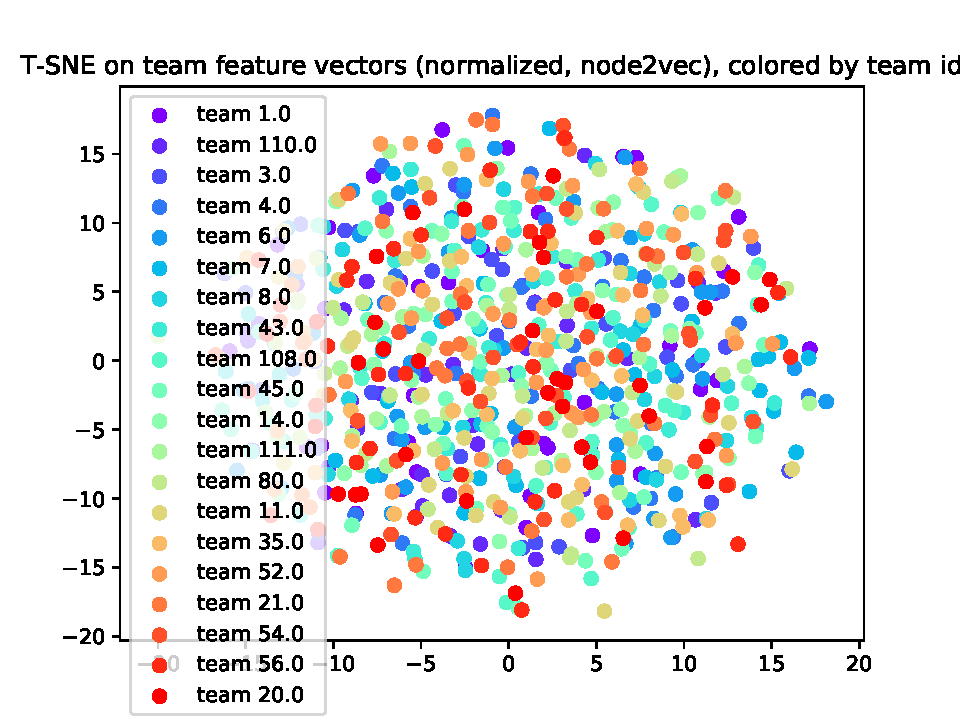
\includegraphics[width=0.45\textwidth]{plots/node2vec_NORM_game_team_teamId_tsne.pdf}
  \caption{T-SNE without confounding features illustrates game result and team styles are hard to predict with current feature vectors.}
    \label{fig:tsne_team}
\end{figure}


\subsection{Game Result Prediction using Feature Vectors}
Despite the t-SNE results showing minimal predictive power for the current feature vectors, we implemented a simple logistic regression (LR) model that modelled multinomial game outcome based on a concatenation of home team and away team's feature vectors. We employed stratified sampling based on team ID to ensure each team had fair representation both in the training dataset of 304 matches and testing set of 76 matches. 

For simple feature vectors, the LR test set accuracy was 43\% and 48\% on training data. For node2vec features, the performance was similarly bad, with test set accuracy of 38\%. 

As a sanity check of our LR implementation, including the goal differential to predict game outcome yielded 100\% accuracy, but obviously this variable cannot be used. Overall, our results indicate we needed richer features, need to learn higher order interactions between players, and incorporate data from many other leagues besides the EPL. Our whole soccer analysis pipeline is available on GitHub at \texttt{\url{https://github.com/ehuang2831/Soccer_Network.git}}.

\begin{figure}[h]
  \label{fig:results_table}
  \centering
    \begin{tabular}{l | l | l}
        \rowcolor{gray!20}
        Features & Predictor & Test Accuracy  \\
        \noalign{\smallskip}\hline\noalign{\smallskip}
        \rowcolor{green!20}
        Simple &  Logistic & 43\% \\
        \rowcolor{blue!20}
        node2vec &  SVM & 47\% \\
        \rowcolor{purple!20}
        Graph CNN & GCN Softmax & 62 \% \\ 
    \end{tabular}
  \caption{Overall results illustrating various node feature embeddings and their predictive power for game prediction outcome. Graph CNNs provide the best test set accuracy, but still are not highly accurate predictors of soccer game outcome, which is a complex problem.}
    \label{fig:results_table}
\end{figure}




\section{Graph Convolutional Neural Network}
%%%%%%%%%%%%%%%%%%%%%%%%%%
\label{sec:graph_GCN}
Given the poor results using standard feature extraction techniques and simple models, we see a few issues to tackle:

\begin{enumerate}

    \item Feature learning on the graph can not just be averaging of individual node features. A soccer team should be classified by the movement from specified nodes to other nodes. Simple features thus don't work. 


    \item The nodes within a soccer team are different from the nodes of other teams. Therefore node2vec does not generalize across teams, requiring a different feature extraction method when using random walks. 


    \item Simple models such as linear regression are not enough. Given the high complexity of networks and the relationship with game results, a more complex model such as neural networks is needed. 

\end{enumerate}

Thus we turn to a new method. Using related work on GCNs [2,6] as inspiration, we created a GCN model that iterates a ``sliding window'' across different paths within a network. 

\subsection{Construction of GCN Data}

We constructed numerous types of data to train on a GCN. Our initial idea was to measure the top-3 hops. That is, we create a vector composing the assigned node, the top 3 nodes that first node links to (in terms of passing rate), then the 9 nodes connected to those top 3 nodes. The resulting vector is of length 13 and can contain information regarding the node itself. We decided to use shot rate, loss rate, gain rate, and average pass rate to categorize the nodes. We then repeated this function for all nodes within the graph, giving us a 17x13x4 matrix for each datapoint. However, this construction had issues. 

One issue is that we are only considering top-3 hops for every graph. In reality, there may be important information in longer path lengths. Additionally, top-3 hops has the potential to only see a subset of nodes within the graph. Lastly taking a vector for each start node does not generalize well across different graphs given different number of players/player types. Simple running of the data on a simple CNN resulted in poor accuracies and losses. We therefore decided to think of a new construction that: 

\begin{enumerate}
    \item Considers all the nodes in some function when creating vectors.

    \item Generalizes better across different teams/graphs. 
\end{enumerate}

\subsection{Novel approach applying random walks and GCNs}
Our final data construction took inspiration from node2vec's random walk procedure, and Gibbs sampling [8]. Like node2vec, we simulate a random walk throughout the network but start at the ``Gain'' state. This is essentially the path of the ball during some possession.  We then assemble the data for each node along this random walk and add it to the datapoint. We repeat this for 100 steps and 100 trials, giving us a 100x100x4 matrix (similar to Gibb's sampling approaches). We can then use this 100x100x4 matrix as a representation of a graph. Given the randomness of the path sampling, this method should generalize well across epochs of training. Additionally, starting at the ``Gain'' state makes each graph consistent. Consistent sizing (100x100) also simplifies the implementation of the GCN. The intuition behind different types of random walks the GCN should discriminate between is illustrated in Figure \ref{fig:intuition}.


\begin{figure}[h]
  \centering
  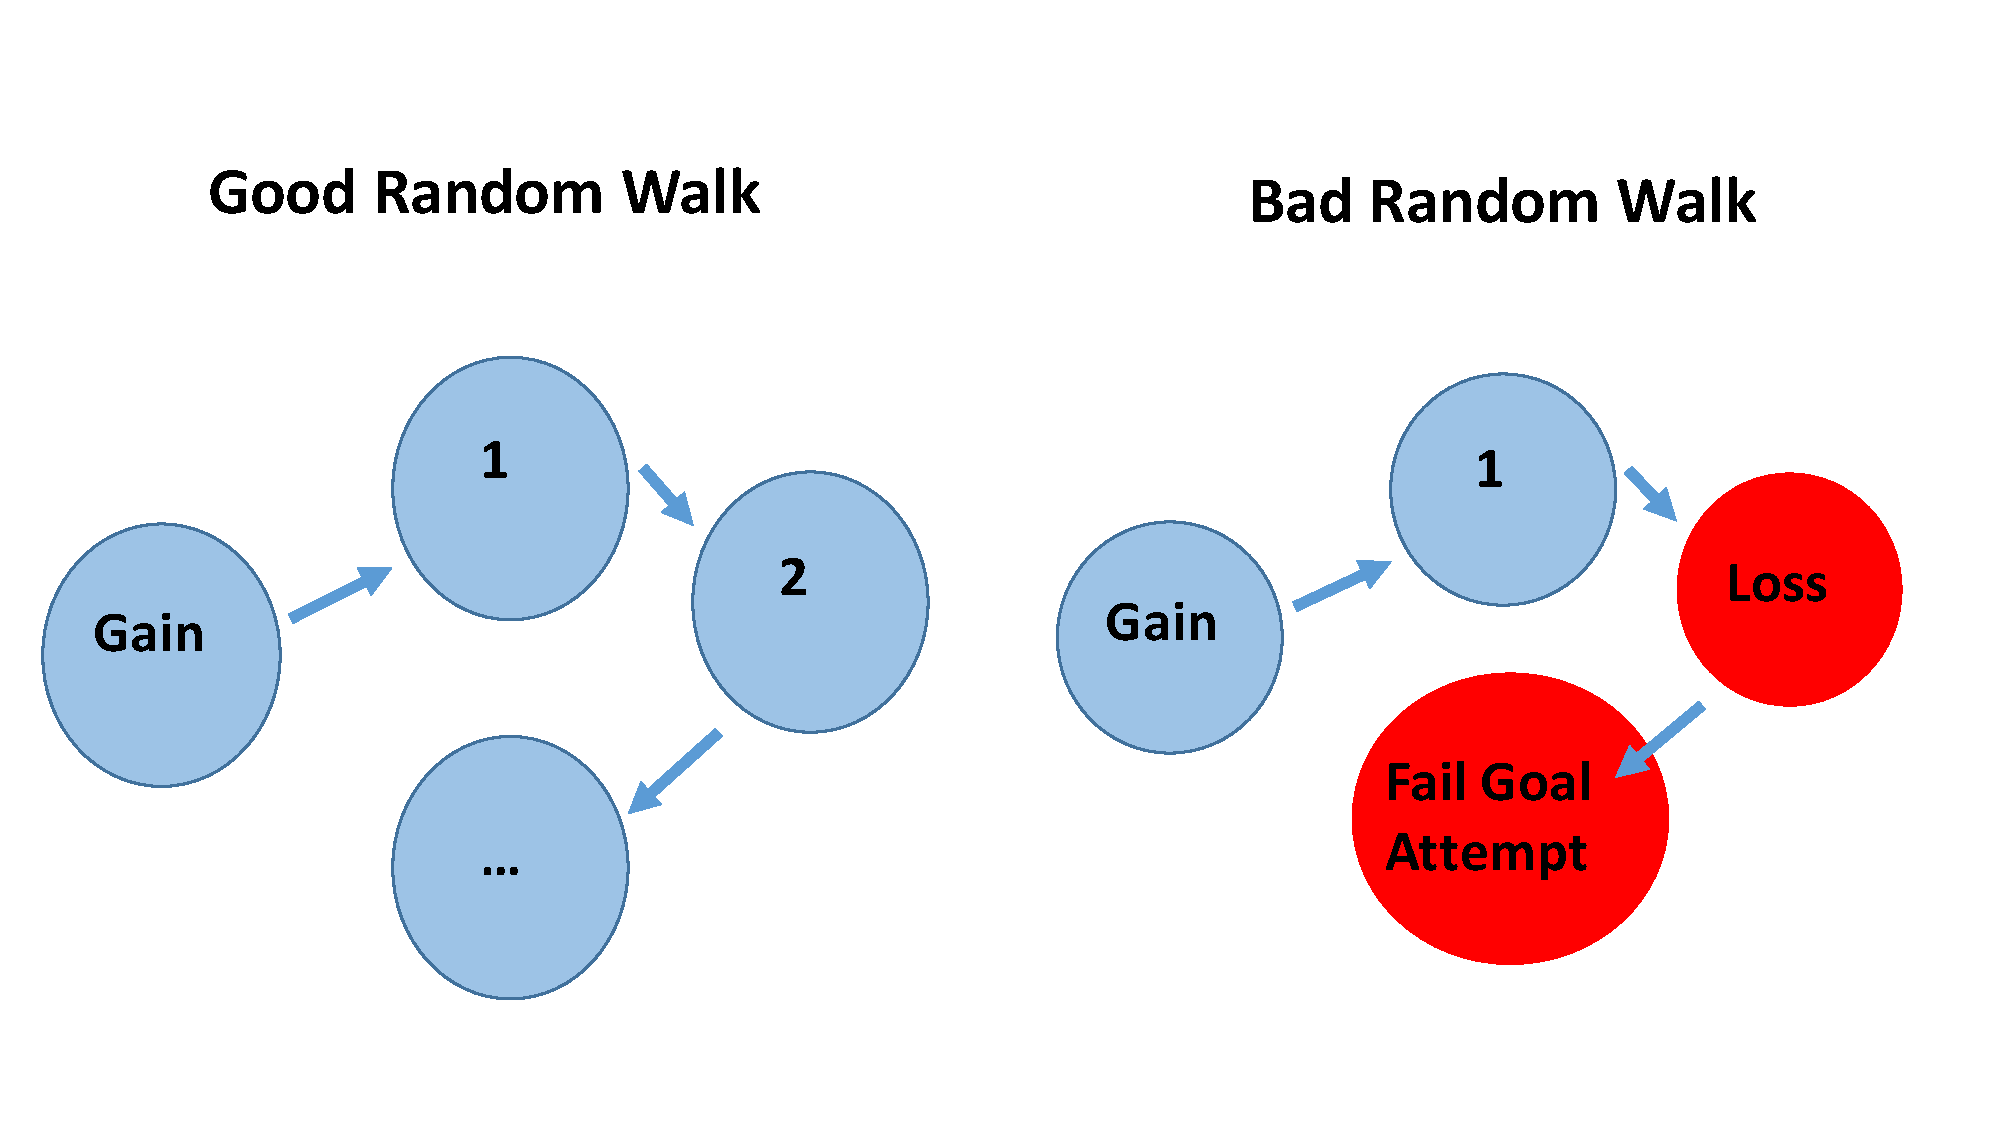
\includegraphics[width=0.45\textwidth]{plots/graph_CNN_intuition.pdf}
  \caption{We designed a \textit{novel} application of random-walks to GCNs that attempts to distinguish ``good paths'' where a team stays in possession (left) from ``bad paths'' where it quickly turns over the ball or fails to score within a long random walk (right). We use domain-specific insight to always start from ``Gain'' nodes where the team just got the ball and had the best chance of continuing its possession.}
  \label{fig:intuition}
\end{figure}

Given our data construction, we now need a GCN implementation that makes sense. We use the generic structure in CNNs: a number of convolutional layers with pooling, then fully connected layers. For our response we use win, loss, or draw. Given the random path data construction, we are trying to learn how different types of n-hop paths contribute to game results. We therefore use a non-traditional sliding window of $(1,n)$ to learn this. This sliding window does not work on multiple paths at the same time, as we want parameter sharing across individual paths in each datapoint. The aggregation comes in the pooling layers where both average pooling and max pooling were tested. Our model architecture is shown in Figure \ref{fig:GCN_architecture}.




%\begin{enumerate}
%    \item Convolutional Layer with 20 filters and (1,10) size sliding window
%    \item RELU transform
%    \item Average pooling of size 4
%    \item Convolutional Layer with 15 filters and (1,5) size sliding window
%    \item RELU transform
%    \item Average pooling of size 2
%    \item Convolutional Layer with 10 filters and (1,3) size sliding window
%    \item RELU transform
%    \item Fully Connected Layer
%    \item RELU transform
%    \item Fully Connected Layer
%    \item RELU transform
%    \item Fully Connected Layer
%    \item Softmax Layer
%\end{enumerate}

\begin{figure}[h!]
  \centering
\begin{tabular}{l |}
    \rowcolor{gray!20}
    Custom GCN Architecture \\
    \rowcolor{blue!20}
    \pbox{20cm}{Conv. Layer with 20 filters and \\ (1,10) size sliding window} \\
    \rowcolor{green!20}
    RELU transform \\
    \rowcolor{blue!20}
    Average pooling of size 4 \\
    \rowcolor{green!20}
    \pbox{20cm}{Conv. Layer with 15 filters and \\ (1,5) size sliding window} \\
    \rowcolor{blue!20}
    RELU transform \\
    \rowcolor{green!20}
    Average pooling of size 2 \\
    \rowcolor{blue!20}
    \pbox{20cm}{Conv. Layer with 10 filters and \\ (1,3) size sliding window} \\
    %Conv. Layer with 10 filters and (1,3) size sliding window \\
    \rowcolor{green!20}
    RELU transform \\
    \rowcolor{blue!20}
    Fully Connected Layer \\
    \rowcolor{green!20}
    RELU transform \\
    \rowcolor{blue!20}
    Fully Connected Layer \\
    \rowcolor{green!20}
    RELU transform \\
    \rowcolor{blue!20}
    Fully Connected Layer \\
    \rowcolor{green!20}
    Softmax Layer \\
\end{tabular}
\caption{We implemented a custom GCN architecture to predict game outcome from learned embeddings.}
  \label{fig:GCN_architecture}
\end{figure}

\subsection{GCN Results on Random Path Data:}

The GCN was trained using cross entropy loss, stochastic gradient descent with learning rate 0.02 and momentum 0.8, and 100 epochs with batch size 60. Given these parameters, the training accuracy started at 30\% and slowly moved up to 66\% before dropping back down. This signals potential problems with the optimizer, and a decreasing learning rate should be adopted. On the test set this GCN achieved 62\% accuracy. 

The small difference in training and test accuracy can be explained by the randomness in the data construction. Given the random sampling, the model ends up reading less noise, as each epoch generates more data from the random path sampling. In the end, there is some significant features within the paths that contribute to wins, losses, and draws. Our model achieved better accuracy on losses and wins than draws. Additionally, our model did not assume the differences in wins, losses, or draws to be ordered. 

Our 62\% test accuracy is significantly better than the top accuracy of all other models tested (48\%). This increase can be attributed to a number of changes, including the path sampling for generalization, and the use of a more complex model to read complex signals. Ultimately, we find that there is information in the constructed network that contributes to end of game results. Specifically, there are sub-paths within random walks which signal that a team is performing well or not well given gain, loss, shot, and average pass rates of players. 





\section{Future Work}
%%%%%%%%%%%%%%%%%%%%%%%%%%
\label{sec:future_work}
%We hope to expand our work to get better predictive and analytical results. We see some success with clustering, but want to try additional feature embeddings and clustering methods. One clustering task to be done is the clustering of individual node embeddings to determine player ``roles''. These roles within a network may lead to some predictive power regarding team performance. We can compare the impact of labeling network roles vs. given roles (striker, midfielder, goalkeeper, etc) within the dataset by running different predictive models on them. 
%
%We also hope to implement our initial proposal ideas. That is, we want to use more complicated predictive models that may incorporate nonlinearity in classification. Other graph based models, like graph convolutional neural networks (GCNs) would also be interesting to look at, though may be limited by the dataset size.  

We hope to expand our work to get better predictive and analytical results. Given good results with the GCN, we hope to try different parameter values. A main hindrance to the training was tuning the learning rate. We hope to test different optimizers for better learning rate tuning (Adam for example). 

We also want to expand the graph structures. As of now, we only considered the simple graph structure. In the future we hope to consider the complex structure with the opponent added. Additionally, we want to consider the averaged structure that is based on a season’s worth of games. 







\section{Conclusion}
%%%%%%%%%%%%%%%%%%%%%%%%%%
\label{sec:conclusion}
Rich network structure is inherent to the team game of soccer, which
manifests as time-variant passing rates between players of a team,
and possession changes between opposing teams. Using network structure to predict
game outcomes and learn latent features representing player roles is of prime importance,
since it can help coaches better understand their teams and aid in the large sports
analytics and betting market.

In this paper, we provided a principled analysis of play-by-player soccer
data, starting from graph extraction and using a mixture of domain knowledge and 
unsupervised feature learning to predict game outcomes. As expected, given the
dynamic, unpredictable nature of soccer games, we could not create a highly-accurate
game outcome predictor. Interestingly though, our results illustrate a marked increase
in predictive power if we use Graph Convolutional Networks (GCNs) even with a limited
dataset compared to conventional techniques.



\section{References}
%%%%%%%%%%%%%%%%%%%%%%%%%%
\label{sec:ref}
\begin{enumerate}

\item https://www.sportsbusinessdaily.com/Journal\\
/Issues/2018/04/16/World-Congress-of-Sports/Research.aspx 

\item Kipf, T.N. and Welling, M., 2016. Semi-supervised classification with graph convolutional networks. arXiv preprint         arXiv:1609.02907.

\item Hoang M. Le, Peter Carr, Yisong Yue, and Patrick Lucey. 2017. Data-Driven Ghosting using Deep Imitation Learning. MIT Sloan Sports Analytics Conference

\item Matthew Kerr. 2015. Applying Machine Learning to Event Data in Soccer    http://hdl.handle.net/1721.1/100607

\item Joel Brooks, Matthew Kerr, and John Guttag. 2016. Using machine learning to draw inferences from pass location data in soccer. Stat. Anal. Data Min. 9, 5 (October 2016), 338-349. DOI: https://doi.org/10.1002/sam.11318 

\item Niepert, Mathias, Mohamed Ahmed, and Konstantin Kutzkov. "Learning convolutional neural networks for graphs." International conference on machine learning. 2016.

\item Grover, Aditya, and Jure Leskovec. "node2vec: Scalable feature learning for networks." Proceedings of the 22nd ACM SIGKDD international conference on Knowledge discovery and data mining. ACM, 2016.

\item Hrycej, Tomas. "Gibbs sampling in Bayesian networks." Artificial Intelligence 46.3 (1990): 351-363.

\item Maaten, Laurens van der, and Geoffrey Hinton. "Visualizing data using t-SNE." Journal of machine learning research 9.Nov (2008): 2579-2605.

\item Hsu, Chih-Wei, Chih-Chung Chang, and Chih-Jen Lin. "A practical guide to support vector classification." (2003): 1-16.




\end{enumerate}


%\section*{Acknowledgments}
%\balance
%\bibliographystyle{abbrv} 
%\begin{small}
%\bibliography{ref/soccer_graph.bib}
%\end{small}

\end{document}

